\subsection{Control Theory}
As a subject, \gls{controltheory} is relatively new, and became more relevant during the space race in the 60s \cite{lennartson_2000}. However, the techniques therein have been used for much longer. The Romans used \gls{controltheory} to control the water levels in their aqueducts and it was later used to control the velocity of windmills \cite{ControlTheoryHistory}. Today, \gls{controltheory} is utilised in advanced technical systems, such as cell phone networks and fighter jets.

\Gls{controltheory} deals with dynamic continuous systems and their control. 
A system can be controlled with one of two basic loops. A closed-loop, or feedback-loop, utilises the output of the process to control the system. For an example see figure \ref{fig:closedloop}. An open-loop works without the use of feedback, see figure \ref{fig:openloop}.%% To model systems as diagrams like this is common practice in \gls{controltheory}. EDIT: repetition

\begin{figure}[H]
\begin{subfigure}[t]{0.999\linewidth}
    \centering
    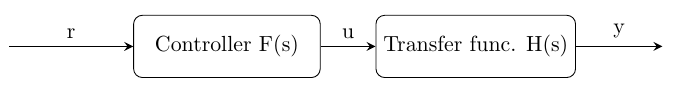
\includegraphics[width=1.0\linewidth]{Theory/nofeedback1.PNG}
    \caption{Block diagram of a system with open loop, without feedback.}
    \label{fig:openloop}\vspace{.4cm}
\end{subfigure}\\
\begin{subfigure}[t]{0.999\linewidth}
    \centering
    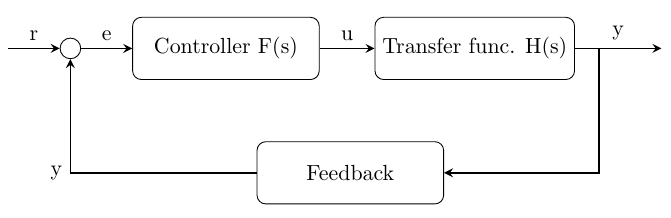
\includegraphics[width=0.999\linewidth]{Theory/feedback1.PNG}
    \caption{Block diagram of system with closed loop, using feedback to control system.}
    \label{fig:closedloop}
\end{subfigure}
\caption{Block diagrams of the general forms of two different loops often used in control theory, the open loop (which can be seen in \subref{fig:openloop}) and the closed loop (which can be seen in \subref{fig:closedloop}).}
\end{figure}
\noindent

\begin{modtext}
These systems are all around us, and the systems where \gls{controltheory} is applied often have disturbances, i.e.~signals that for some unintended reason affects the system. 
If the system was unaffected by these disturbances, it 
\end{modtext} 
%If these disturbances didn't affect the system, the system 
would not need any feedback signals and \begin{modtext}
could thus be modelled using an open loop, see figure \ref{fig:openloop}.
\end{modtext}
%look like the system in figure\ref{fig:openloop}. 
The main objective of \gls{controltheory} is to find 
\begin{modtext}
suitable controllers for signals (with or without feedback) given some condition
\end{modtext}
%a suitable controller for one or more feedback signal given some condition we want to meet 
---like the r signal in figure \ref{fig:closedloop}.
\begin{modtext}
The purpose of this is 
\end{modtext}
to accomplish stable systems, without delay or overshoot. In the course \cite{ERE103} a combination of proportional (P), integral (I) and derivative (D) controllers are used to achieve this goal, \begin{newtext}
resulting in what is commonly referred to as PID-controllers.
\end{newtext} 
\begin{modtext}
When analysing systems, 
\end{modtext}
%When we want to analyse or calculate our systems 
they are often transformed from the time domain to the frequency domain
\begin{modtext}
using the Laplace transform.
\end{modtext}
%which is possible with the Laplace transform.
\begin{newtext}
This is done since the models of the controllers are typically easier to calculate and manipulate when working in the frequency domain.
\end{newtext}